% ============================================================
%  TERM PROJECT – USER MANUAL
%  Databases · THGA Bochum
%
%  How to use the Prevently desktop app once it's installed and
%  connected to a running API. For installation instructions, see
%  documentation.tex (section "Operation and deployment").
% ============================================================
\documentclass[11pt,a4paper]{article}

\usepackage{thga-db}
\usepackage{seqsplit}  % allows line-breaking inside long unbroken \texttt strings (e.g. API paths)
\usepackage{float}     % [H] placement -- keeps each screenshot exactly where it's inserted

\renewcommand{\thgaKurs}{Databases}
\renewcommand{\thgaDatum}{Summer Term 2026}

\begin{document}
\thispagestyle{empty}
\thgaTitel{Prevently -- User Manual}%
{How to use the desktop app}

\begin{infobox}
\textbf{Author:} Anton Möller \\
\textbf{Module:} Introduction to Database Management Systems · THGA Bochum \\
\textbf{Stack:} PostgreSQL · FastAPI · Docker Compose · tkinter (\texttt{.deb}) \\
\textbf{Repository:} \url{https://github.com/Antonmlr/Prevently}
\end{infobox}

\tableofcontents
\vspace{1em}

% ============================================================
\section{Introduction}
% ============================================================


This manual is for all users of the Prevently desktop application. It provides a short guide on how to use the app
on your local machine after it has been installed and connected to the running API. This application allows users to manage
there medical checkups without a user account. Users can check which checkups are due, book appointments, 
mark checkups as completed, and find doctors who perform specific checkups near them.

% ============================================================
\section{Starting the app}
% ============================================================

After starting the app, a connection dialog will appear and asking for the API URL and an X-API-Key. The API URL 
is the address of the running API, which is connected to the database. If you are using the database on you local machine, 
the API URL is \texttt{http://localhost:8000}. The X-API-Key is a secret key that is used to authenticate the user and is needed 
to access the POST API endpoints (write into database). The X-API-Key is in the .env file and is provided by your local admin 
or yourself running the project.

\begin{figure}[H]
  \centering
  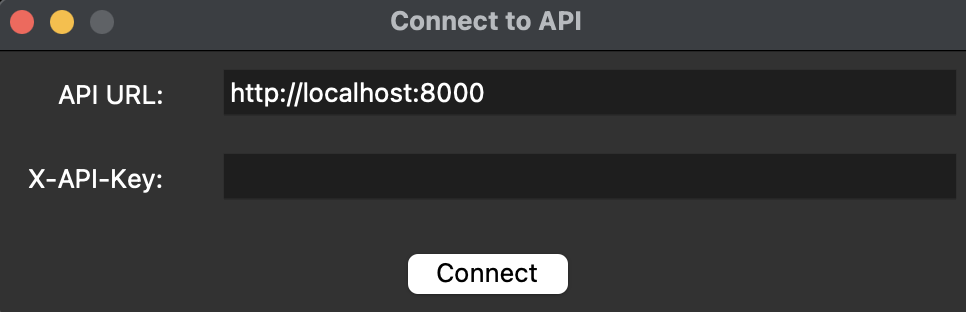
\includegraphics[width=0.85\linewidth]{assets/connection.png}
  \caption{Connection dialog for the Prevently desktop app.}
  \label{fig:connection}
\end{figure}

% ============================================================
\section{Overview of the screens}
% ============================================================

Once your connection is established, the dashboard of the desktop app will appear. There you have an overview of. checkups for a
selected user and you have the opportunity to mark a checkup as completed. The details tab allows you to create a new user and book an appointment for a due checkup. 
In the feature screen you can search for a doctor and see which checkups are covered by an insurance provider.

\subsection{Dashboard}

\begin{figure}[H]
  \centering
  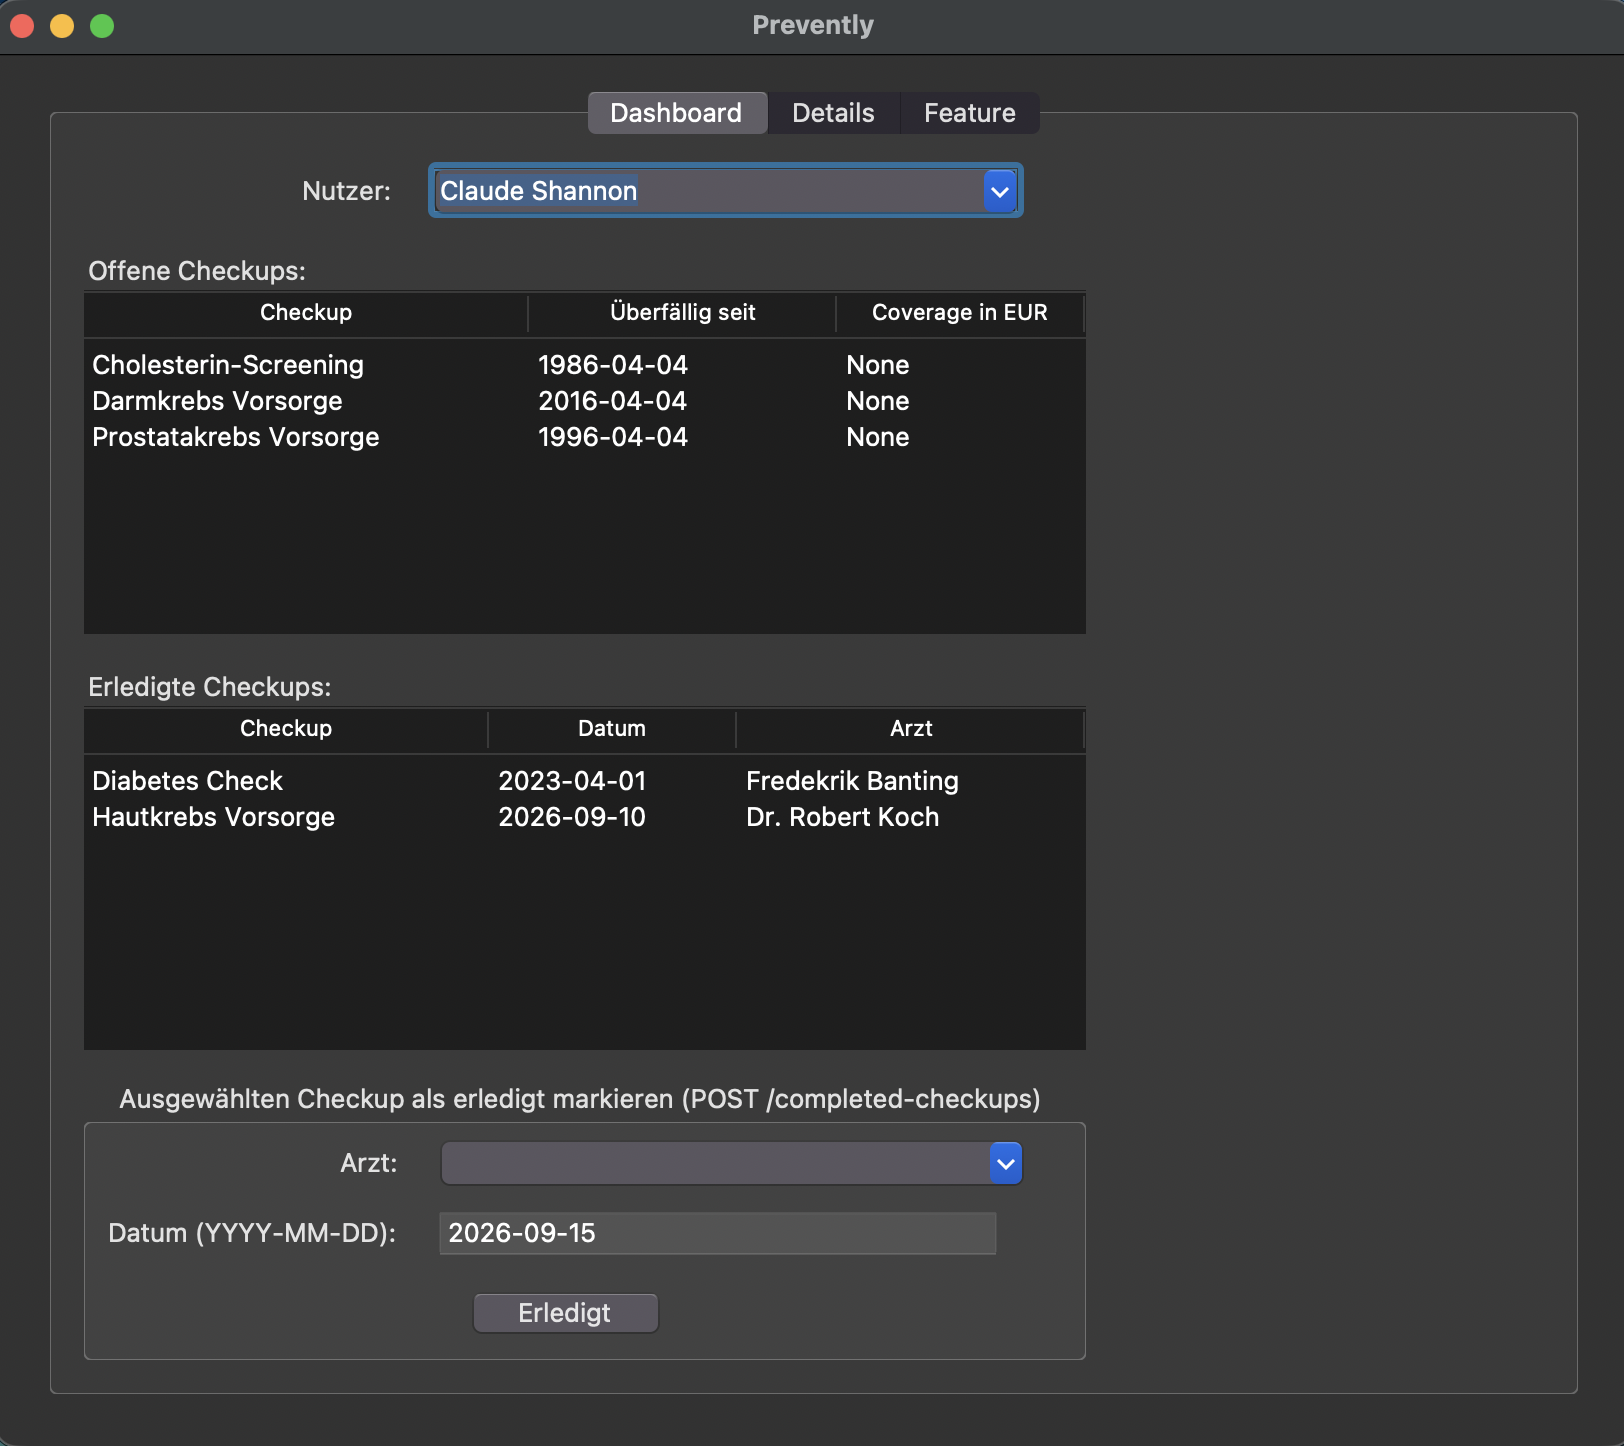
\includegraphics[width=0.85\linewidth]{assets/Dashboard.png}
  \caption{Main dashboard}
  \label{fig:dashboard}
\end{figure}

The dashboard allows to filter for a selected  user and shows the due checkups and already completed checkups. 
If you completed a due checkup, please select the checkup from the due checkups list and then select in the table 
below a doctor and date. After that, click on "Erledigt" to mark the checkup as completed. Than the checkup will appear at the 
completed checkup table.

\subsection{Details}

\begin{figure}[H]
  \centering
  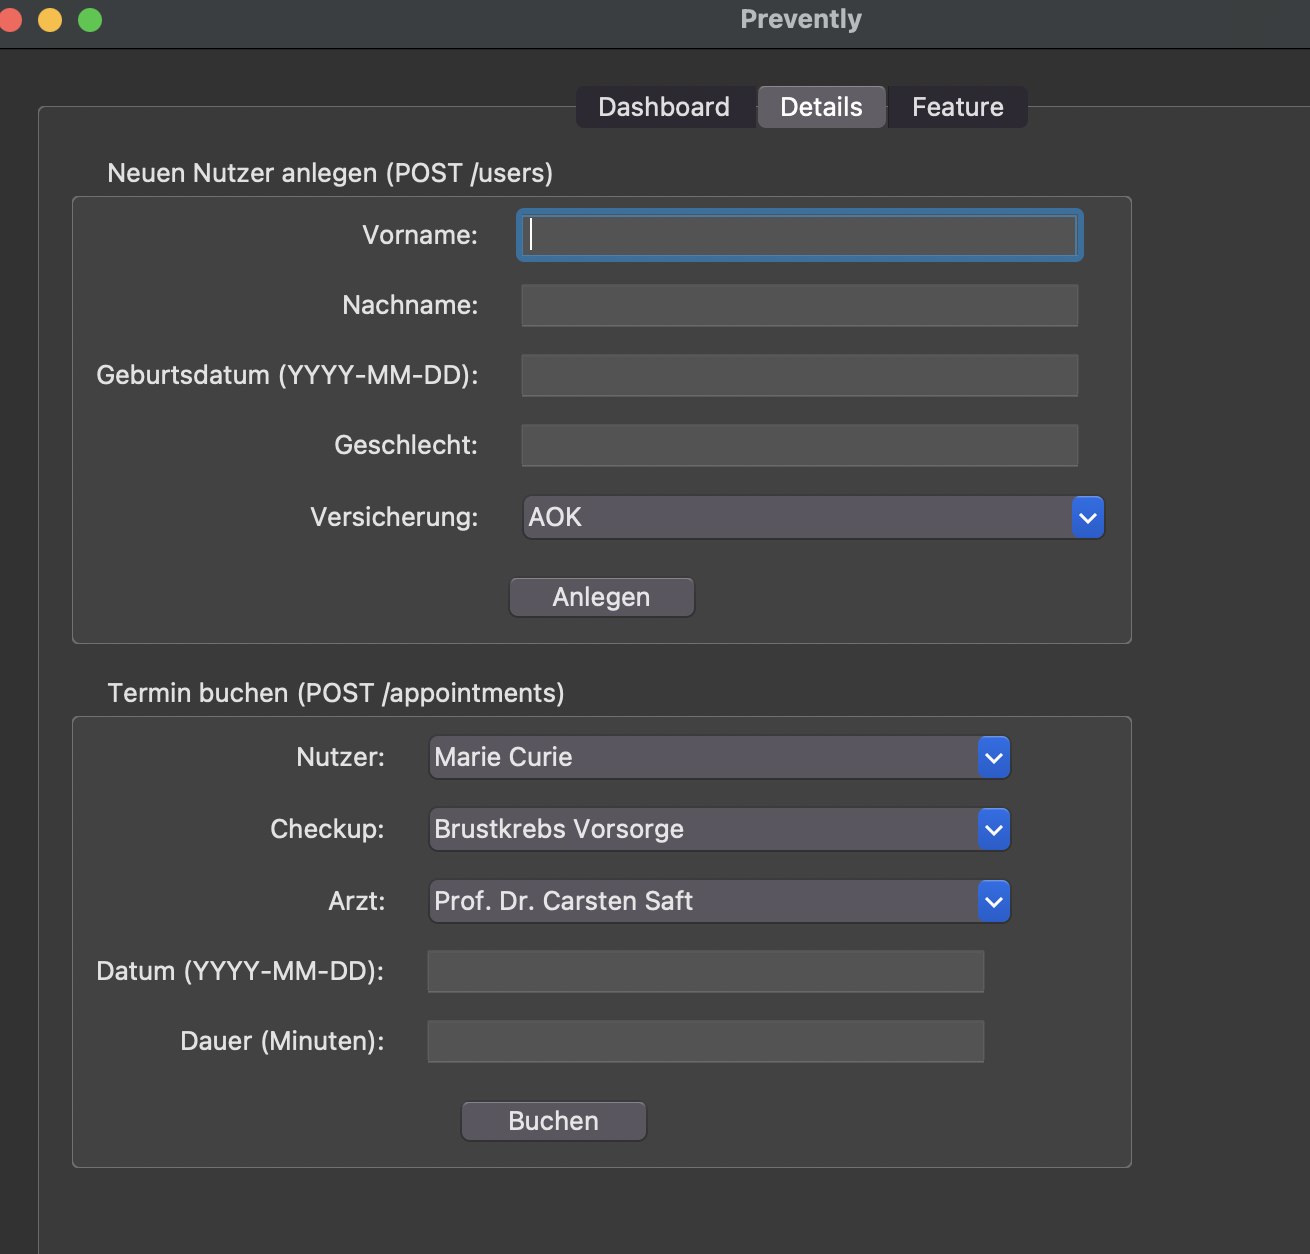
\includegraphics[width=0.85\linewidth]{assets/Details.png}
  \caption{Details Screen to add user and book appointments}
  \label{fig:details}
\end{figure}

If you would like to create a new user or book an appointment, this can be done in the details screen. To create a new user 
fill in all shown fields and select an insurance. Then click on "Anlegen" and the user is added to the database. Please note 
that you fill in the date in the shown format and that the database at the moment only support male and female as gender. 
To book an appointment you can select the user and also the checkup with the doctor you would like to have the appointment for. 
At the moment the appointment is only created in the database and not shown in the app. This will be implemented in the next releases.


\subsection{Feature}

\begin{figure}[H]
  \centering
  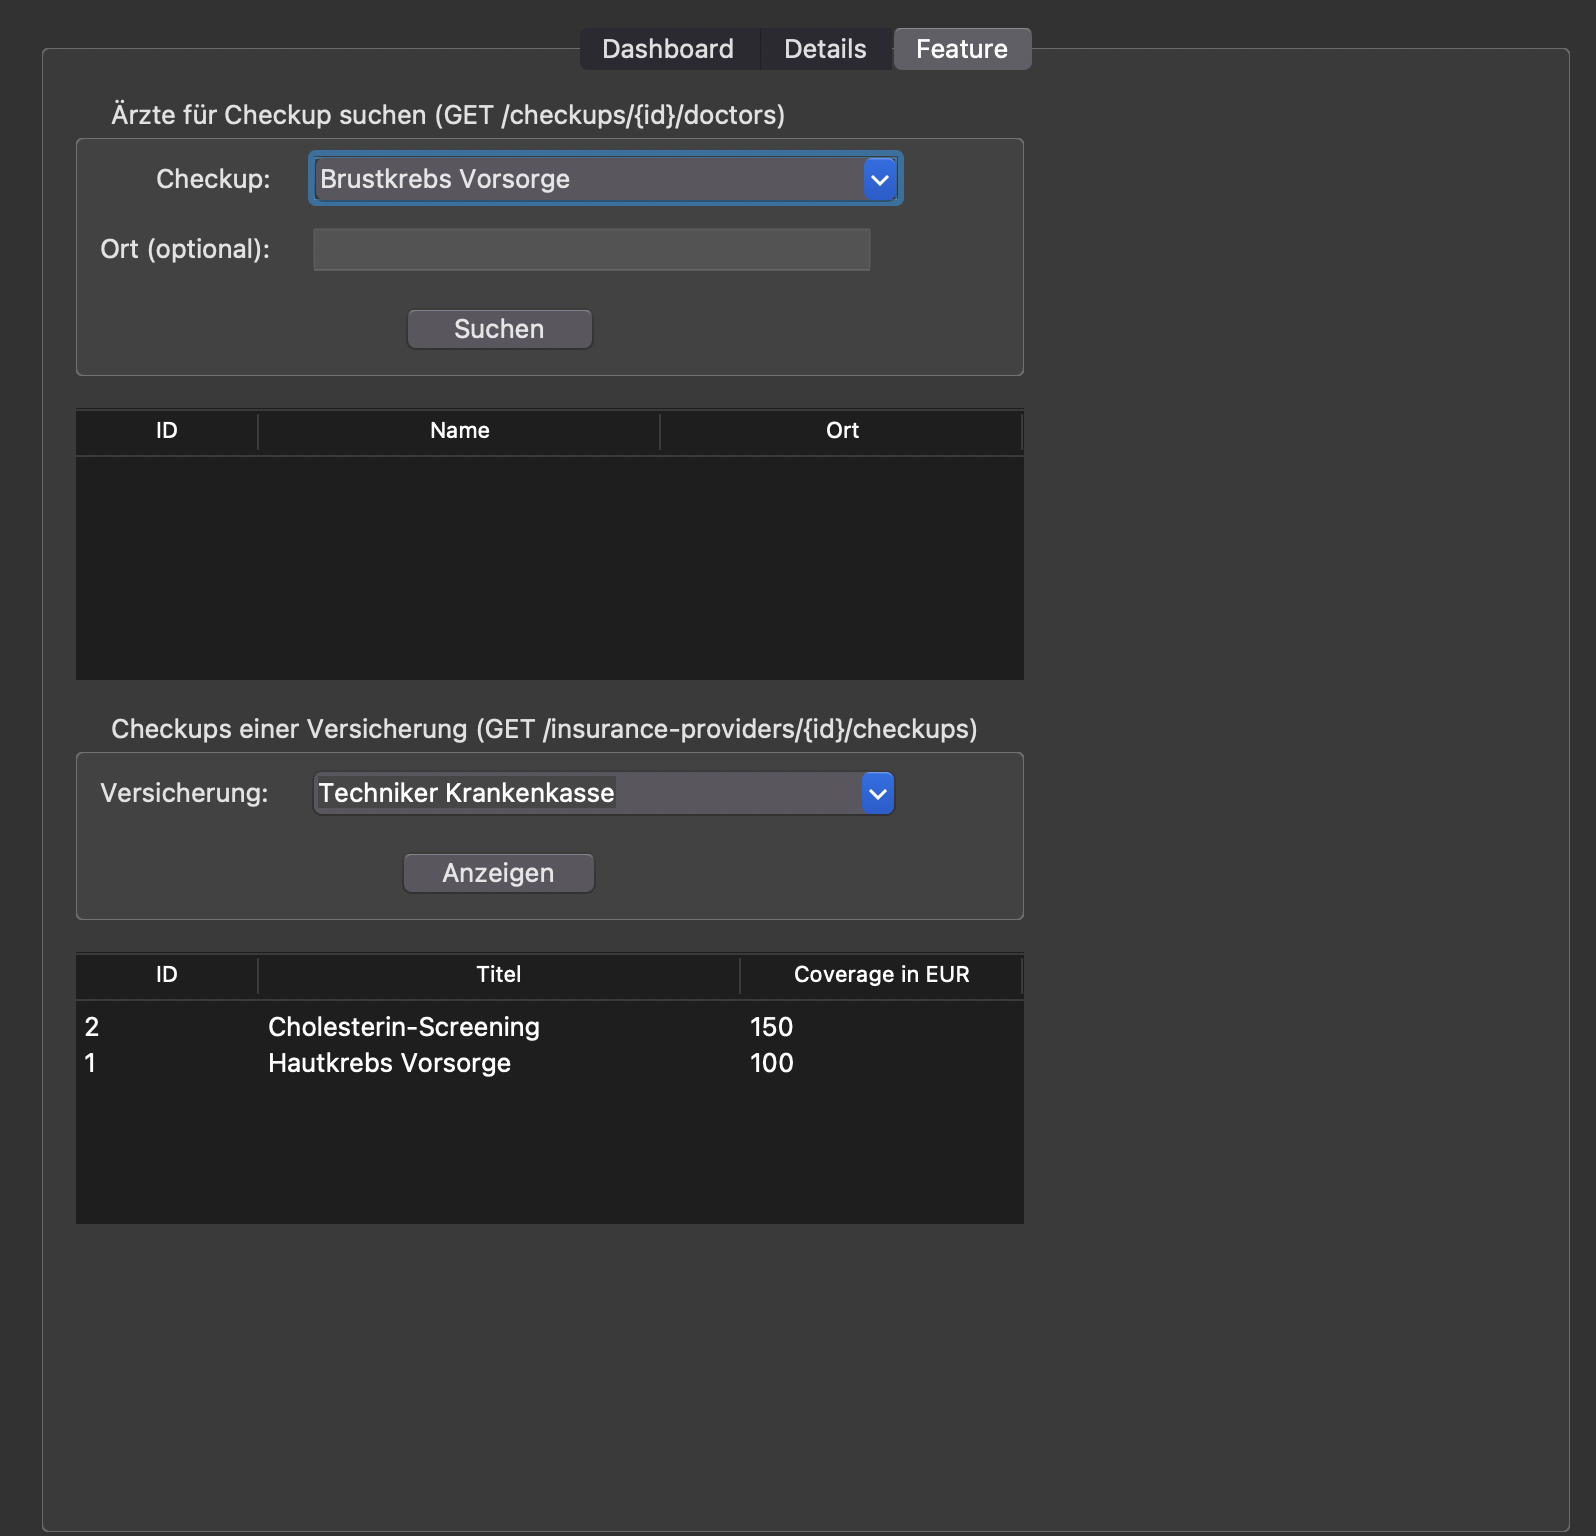
\includegraphics[width=0.85\linewidth]{assets/Feature.png}
  \caption{Feature Screen to search for doctors and also lookup the coverage}
  \label{fig:feature}
\end{figure}

In the Feature Screen you can search for a doctor in a specific city. The location field in the UI is optional. With the second table 
you can see which checkups a selected insurance provider covers.

\end{document}
